% =============================================================================
% Section 1.3: Project Outcomes
% =============================================================================

\section{Project Outcomes}
\label{sec:project-outcomes}

The successful completion of this graduation project yields tangible deliverables demonstrating functional completeness, architectural discipline, and operational readiness. Outcomes span executable software, persistent data models, deployment automation, machine-readable API contracts, automated test suites, and human-readable architecture documentation. Each outcome is traceable to one or more objectives in Section~\ref{subsec:project-objectives}.

\subsection{Primary Software Artefact: NestJS REST API}
\label{subsec:outcome-api}

The centrepiece deliverable is a fully functional NestJS~10 application written in TypeScript, exposing more than \textbf{150 REST endpoints} across \textbf{twenty registered modules}: sixteen domain modules (Auth, Courses, Enrollment, Payments, Media, AI Pipeline, Assessment, Discussion, Progress, Reviews, Certificates, Search, Streak, Notifications, Instructor, Admin) and four infrastructure modules (Prisma, Events, Audit, plus shared Common utilities). Controllers remain thin, delegating to application-layer use cases; domain rules live in entities and domain services; infrastructure concerns (Prisma repositories, Stripe client, Mux adapter, email sender) implement ports defined inward.

Representative endpoint families include:
\begin{itemize}
  \item \textbf{Auth} --- signup, verify-email, login, refresh, logout, forgot/reset password, profile;
  \item \textbf{Courses} --- CRUD courses/modules/lessons, reorder, publish, instructor-scoped listing;
  \item \textbf{Enrollment} --- create pending enrollment, activate from payment, cancel, list my enrollments;
  \item \textbf{Payments} --- create PaymentIntent, Stripe webhook receiver, refund request;
  \item \textbf{Media} --- request Mux upload URL, webhook handler, assign video to lesson, signed playback;
  \item \textbf{Assessment} --- create quizzes/questions, start/submit attempts, async grading callbacks;
  \item \textbf{Progress} --- mark lesson complete, course progress summary, certificate eligibility;
  \item \textbf{Discussion} --- create threads/posts, moderation accept/reject, list by lesson;
  \item \textbf{Search} --- full-text course search, category management;
  \item \textbf{Instructor/Admin} --- analytics dashboards, audit log queries, user administration.
\end{itemize}

All public endpoints are documented via Swagger decorators; request DTOs use \texttt{class-validator} for input validation; authorisation guards enforce JWT presence and role permissions consistently.

\subsection{PostgreSQL Database Schema and Migration History}
\label{subsec:outcome-database}

The persistent data model comprises \textbf{58 Prisma models} mapped to normalised PostgreSQL tables, including core entities (\texttt{User}, \texttt{Course}, \texttt{Module}, \texttt{Lesson}, \texttt{Enrollment}, \texttt{Payment}, \texttt{VideoAsset}, \texttt{Quiz}, \texttt{QuizAttempt}, \texttt{LessonProgress}, \texttt{DiscussionThread}, \texttt{Review}, \texttt{Certificate}, \texttt{OutboxMessage}, \texttt{PipelineJob}) and supporting join/index tables for RBAC, idempotency records, refresh tokens, and audit events. Foreign-key constraints preserve referential integrity; strategic indexes support search vectors, instructor analytics queries, and outbox polling patterns.

The full \textbf{Prisma migration history} chronicles schema evolution from initial bootstrap through incremental feature additions (payments hardening, outbox indexes, AI job tracking). Migrations enable reproducible provisioning via \texttt{prisma migrate deploy} in Docker Compose, CI pipelines, and evaluator local setups---satisfying the faculty criterion that an interested reader could rebuild the database layer without manual DDL execution.

\subsection{Deployment and Operations Stack}
\label{subsec:outcome-deployment}

NexaLearn ships with \textbf{Docker Compose} orchestration defining services for the API container, PostgreSQL~15, Redis~7, and an \textbf{Nginx} reverse proxy. Nginx terminates TLS in production-oriented configurations, forwards proxied requests to NestJS, enforces client body size limits for uploads, and applies rate limiting backed by Redis when configured. Environment variables externalise secrets (Stripe keys, Mux tokens, JWT secrets, database URLs) following twelve-factor principles.

The deployment outcome enables evaluators to launch the entire stack with minimal manual dependency installation and provides a credible path toward cloud deployment (e.g., AWS ECS, Railway, or DigitalOcean App Platform) without architectural rework.

\subsection{OpenAPI Documentation and Developer Experience}
\label{subsec:outcome-openapi}

NestJS Swagger integration auto-generates an \textbf{OpenAPI~3.0 specification} served at \texttt{/api/docs}, documenting paths, request/response schemas, authentication schemes (\texttt Bearer JWT), and standard error envelopes. This contract reduces frontend integration friction, supports codegen for client SDKs, and serves as a living reference validated against controller decorators during continuous integration.

\subsection{Automated Test Suite}
\label{subsec:outcome-tests}

Verification artefacts include unit tests for domain entities and use-case logic, and \textbf{17+ integration test files} leveraging \textbf{Testcontainers} to spin ephemeral PostgreSQL instances (and Redis where required). Critical scenarios under automated regression include:
\begin{itemize}
  \item concurrent outbox processor workers without duplicate side effects;
  \item Stripe webhook idempotency and enrollment activation;
  \item payment expiration of pending enrollments;
  \item progress projection updates upon \texttt{LessonCompleted} events;
  \item course access control denying unenrolled playback;
  \item Mux webhook asset state transitions;
  \item auth refresh token rotation and reuse invalidation.
\end{itemize}

These tests provide confidence that cross-bounded-context workflows---the primary source of production bugs in event-heavy systems---behave correctly under conditions difficult to exercise manually.

\subsection{Architecture and Project Documentation}
\label{subsec:outcome-docs}

Beyond this LaTeX report, the repository includes inline module README fragments, Prisma schema comments, sequence descriptions for payment and AI flows, and TikZ/architecture diagrams. Appendix~D provides selected code walkthroughs; Chapter~4 presents the authoritative system design narrative. Together they satisfy the faculty expectation that the project be \textit{self-contained}: a motivated reader could understand, extend, or rebuild a similar platform without oral defence supplementation.

\subsection{Quantitative Summary of Deliverables}
\label{subsec:outcome-metrics}

Table~\ref{tab:deliverables-metrics} consolidates quantitative metrics for quick reference by evaluators.

\begin{table}[H]
  \centering
  \caption{Quantitative Summary of NexaLearn Project Outcomes}
  \label{tab:deliverables-metrics}
  \small
  \begin{tabular}{@{}lrp{7.5cm}@{}}
    \toprule
    \textbf{Deliverable} & \textbf{Quantity} & \textbf{Notes} \\
    \midrule
    REST API endpoints & 150+ &
    Across auth, courses, commerce, media, AI, analytics \\
    \addlinespace
    NestJS modules & 20 &
    16 domain + 4 infrastructure \\
    \addlinespace
    Bounded contexts & 16 &
    Grouped into 3 high-level modules \\
    \addlinespace
    PostgreSQL models/tables & 58 &
    Prisma-managed with FK constraints \\
    \addlinespace
    Integration test files & 17+ &
    Testcontainers-backed PostgreSQL \\
    \addlinespace
    External integrations & 5+ &
    Stripe, Mux, AWS S3, Redis, AI workers \\
    \addlinespace
    Docker Compose services & 4 &
    API, PostgreSQL, Redis, Nginx \\
    \bottomrule
  \end{tabular}
\end{table}

\begin{figure}[H]
  \centering
  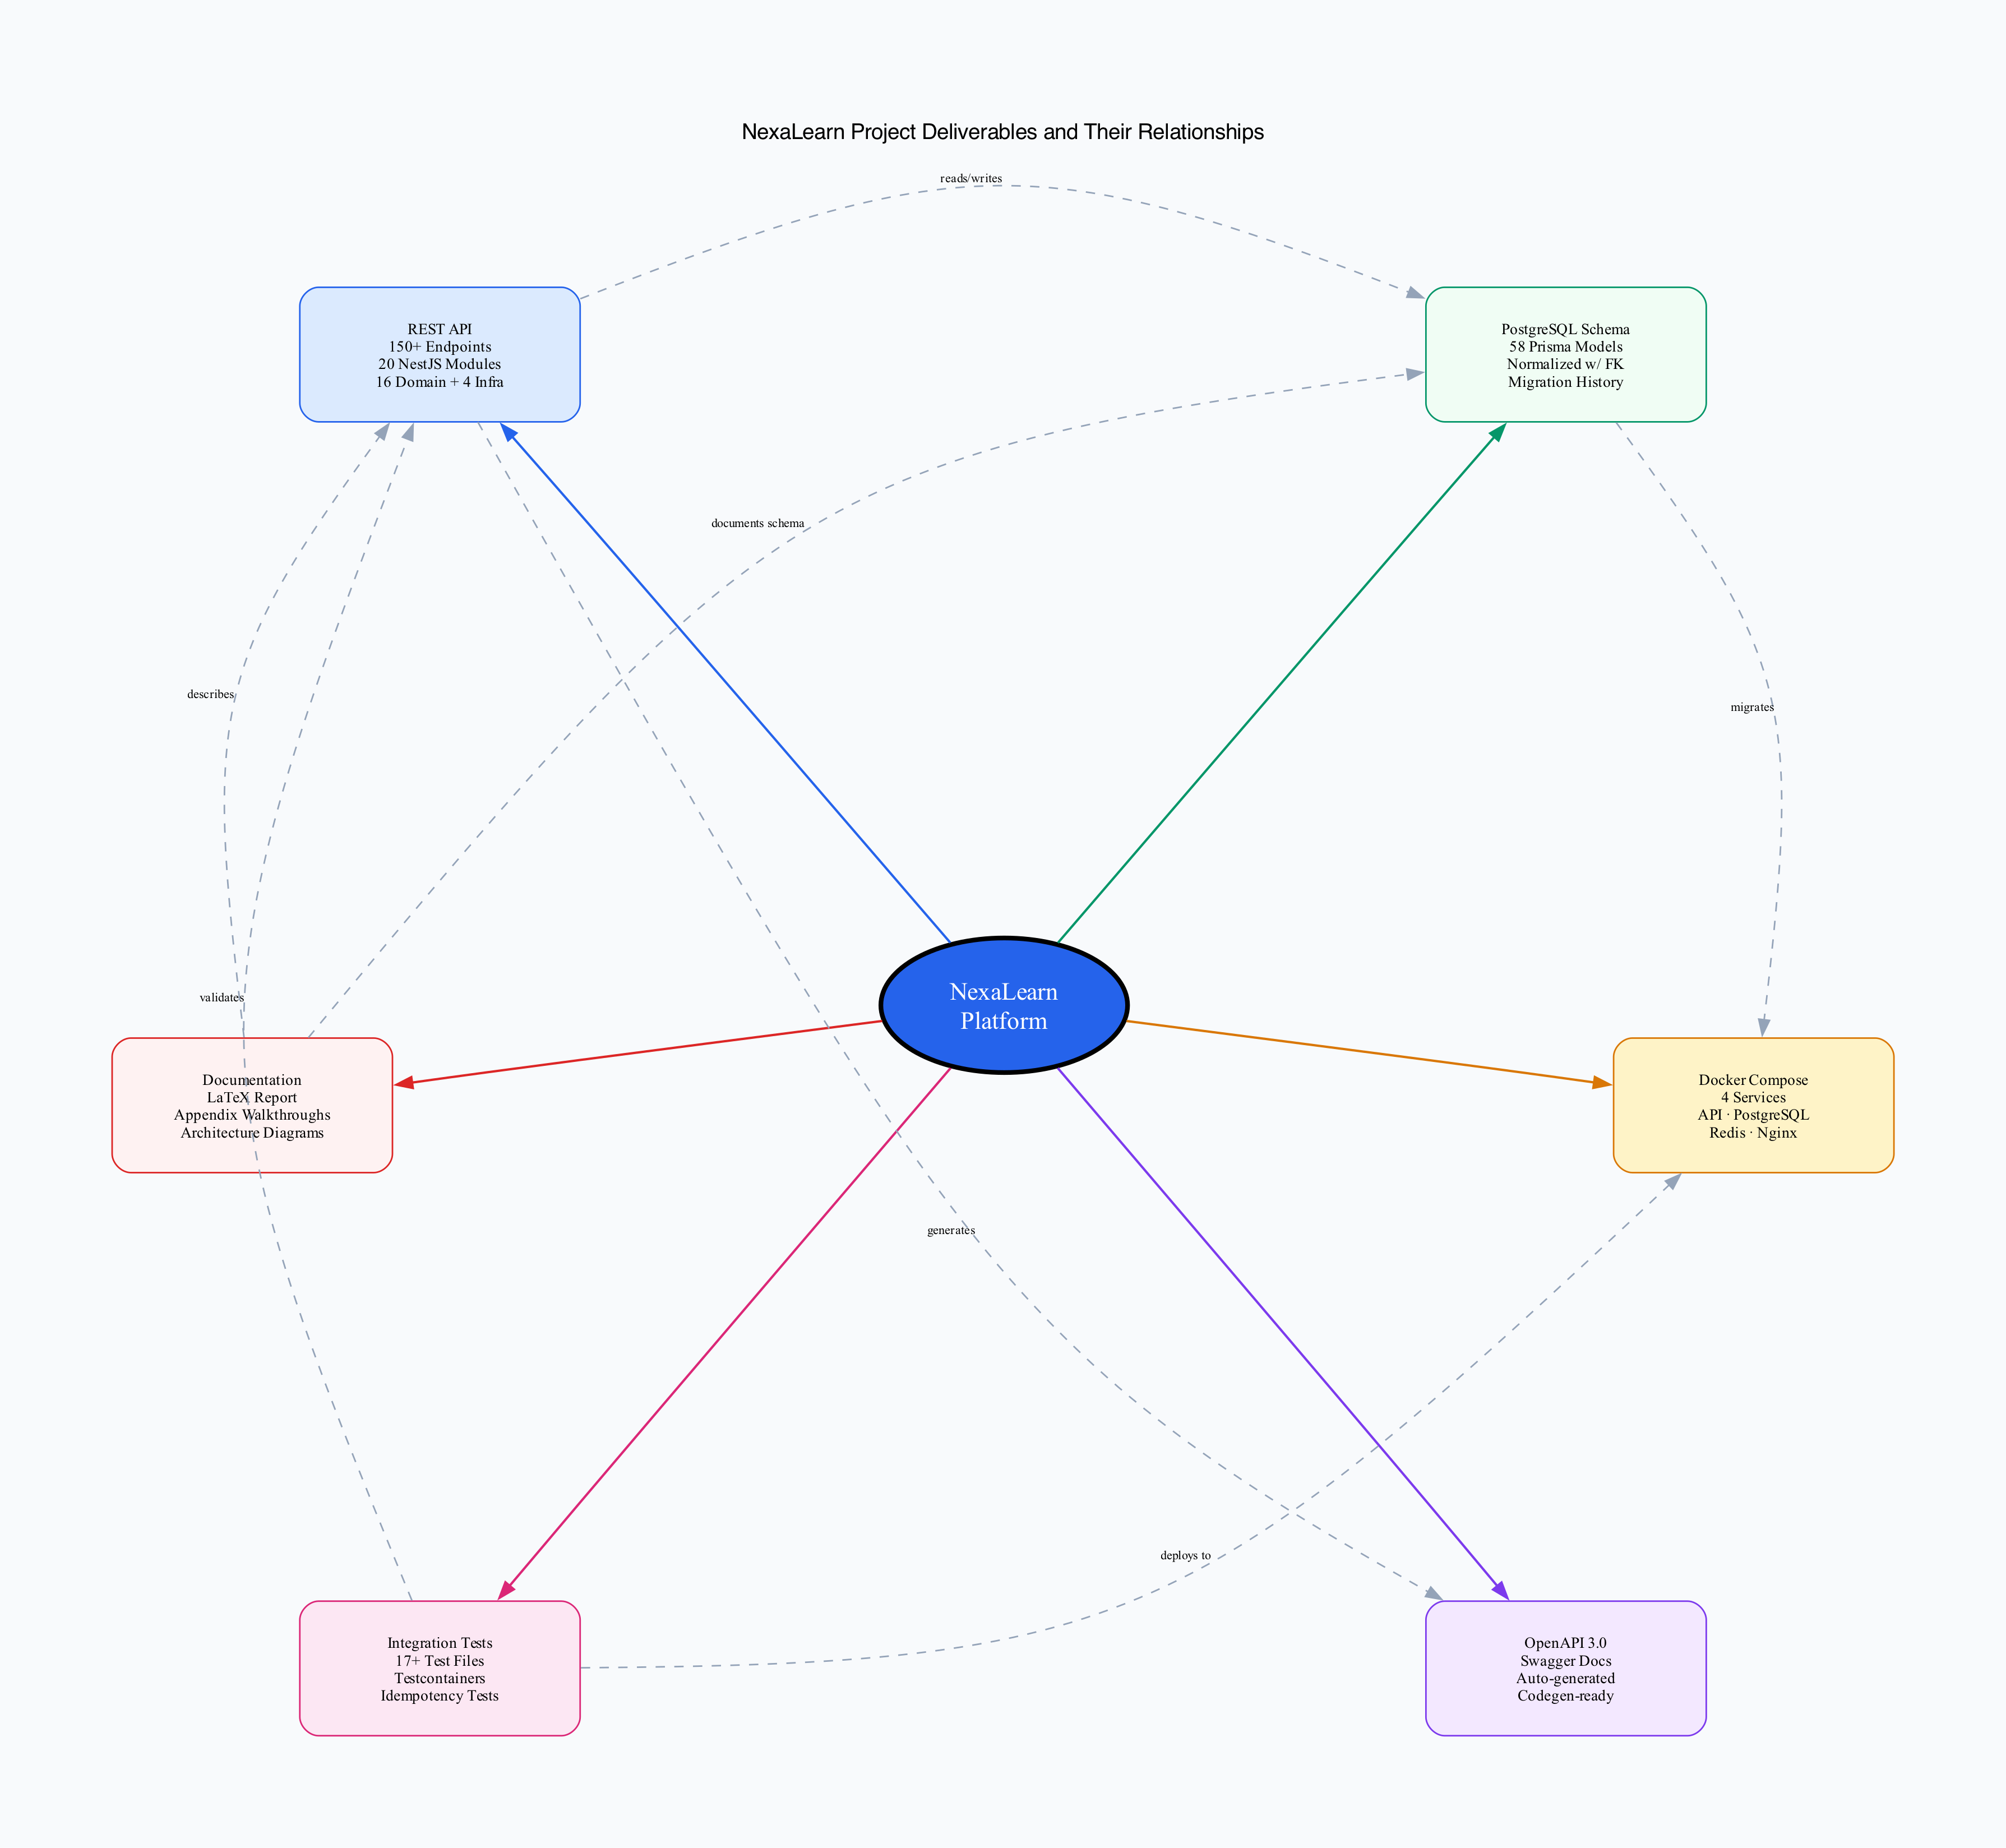
\includegraphics[width=0.90\textwidth]{images/deliverables_overview.png}
  \caption{Summary of NexaLearn Project Deliverables and Their Relationships}
  \label{fig:deliverables-overview}
\end{figure}

Figure~\ref{fig:deliverables-overview} illustrates dependencies among deliverables: the API implements business logic against the schema; migrations version the schema; Docker Compose deploys API and dependencies; OpenAPI documents the API surface; integration tests validate cross-module behaviour; and this report plus appendices capture design intent. Each outcome closes the loop between motivation (Section~\ref{sec:motivation}), problem definition (Section~\ref{subsec:problem-definition}), and objectives (Section~\ref{subsec:project-objectives}).
